% Created by tikzDevice version 0.12.3 on 2020-04-05 20:23:04
% !TEX encoding = UTF-8 Unicode
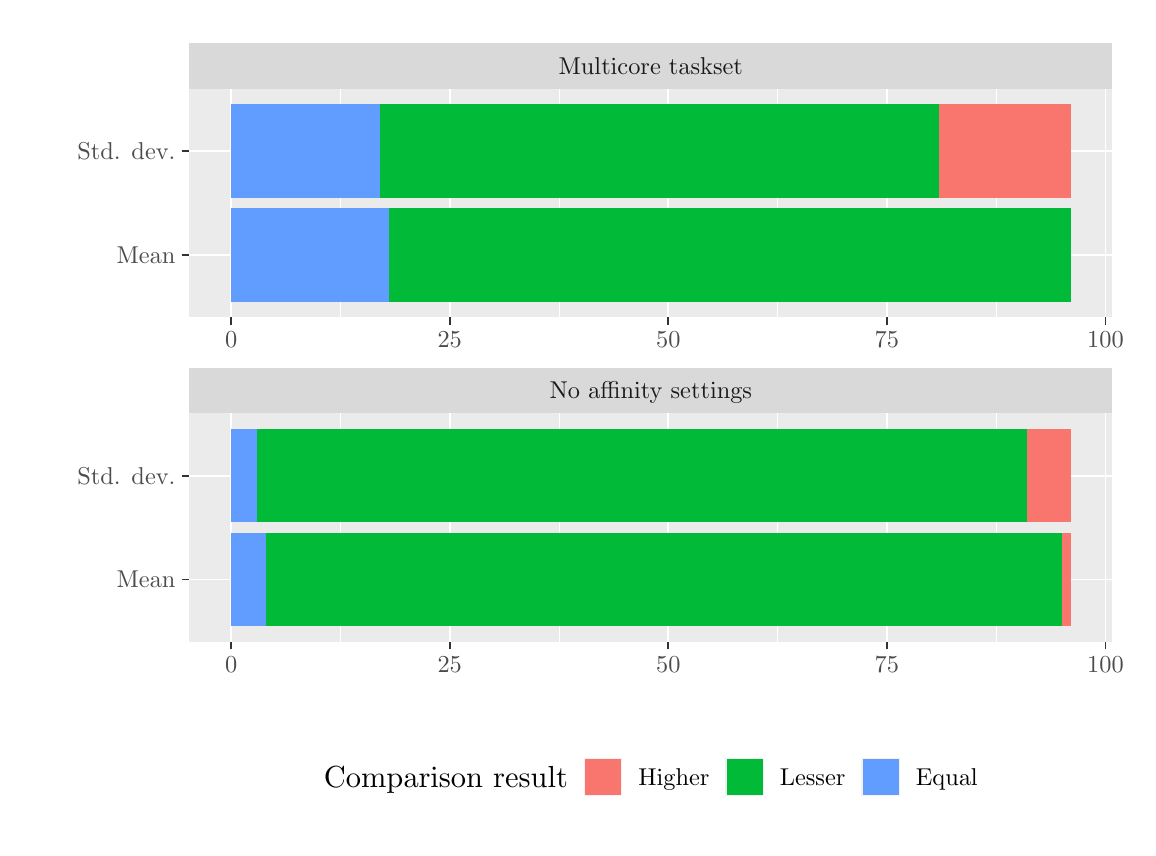
\begin{tikzpicture}[x=1pt,y=1pt]
\definecolor{fillColor}{RGB}{255,255,255}
\path[use as bounding box,fill=fillColor,fill opacity=0.00] (0,0) rectangle (397.48,289.08);
\begin{scope}
\path[clip] (  0.00,  0.00) rectangle (397.48,289.08);
\definecolor{drawColor}{RGB}{255,255,255}
\definecolor{fillColor}{RGB}{255,255,255}

\path[draw=drawColor,line width= 0.6pt,line join=round,line cap=round,fill=fillColor] (  0.00,  0.00) rectangle (397.48,289.08);
\end{scope}
\begin{scope}
\path[clip] ( 58.35,184.47) rectangle (391.98,267.01);
\definecolor{fillColor}{gray}{0.92}

\path[fill=fillColor] ( 58.35,184.47) rectangle (391.98,267.01);
\definecolor{drawColor}{RGB}{255,255,255}

\path[draw=drawColor,line width= 0.3pt,line join=round] (113.01,184.47) --
	(113.01,267.01);

\path[draw=drawColor,line width= 0.3pt,line join=round] (191.99,184.47) --
	(191.99,267.01);

\path[draw=drawColor,line width= 0.3pt,line join=round] (270.98,184.47) --
	(270.98,267.01);

\path[draw=drawColor,line width= 0.3pt,line join=round] (349.96,184.47) --
	(349.96,267.01);

\path[draw=drawColor,line width= 0.6pt,line join=round] ( 58.35,206.98) --
	(391.98,206.98);

\path[draw=drawColor,line width= 0.6pt,line join=round] ( 58.35,244.50) --
	(391.98,244.50);

\path[draw=drawColor,line width= 0.6pt,line join=round] ( 73.52,184.47) --
	( 73.52,267.01);

\path[draw=drawColor,line width= 0.6pt,line join=round] (152.50,184.47) --
	(152.50,267.01);

\path[draw=drawColor,line width= 0.6pt,line join=round] (231.49,184.47) --
	(231.49,267.01);

\path[draw=drawColor,line width= 0.6pt,line join=round] (310.47,184.47) --
	(310.47,267.01);

\path[draw=drawColor,line width= 0.6pt,line join=round] (389.46,184.47) --
	(389.46,267.01);
\definecolor{fillColor}{RGB}{97,156,255}

\path[fill=fillColor] ( 73.52,190.10) rectangle (130.39,223.86);
\definecolor{fillColor}{RGB}{0,186,56}

\path[fill=fillColor] (130.39,190.10) rectangle (376.82,223.86);
\definecolor{fillColor}{RGB}{97,156,255}

\path[fill=fillColor] ( 73.52,227.62) rectangle (127.23,261.38);
\definecolor{fillColor}{RGB}{0,186,56}

\path[fill=fillColor] (127.23,227.62) rectangle (329.43,261.38);
\definecolor{fillColor}{RGB}{248,118,109}

\path[fill=fillColor] (329.43,227.62) rectangle (376.82,261.38);
\end{scope}
\begin{scope}
\path[clip] ( 58.35, 67.14) rectangle (391.98,149.68);
\definecolor{fillColor}{gray}{0.92}

\path[fill=fillColor] ( 58.35, 67.14) rectangle (391.98,149.68);
\definecolor{drawColor}{RGB}{255,255,255}

\path[draw=drawColor,line width= 0.3pt,line join=round] (113.01, 67.14) --
	(113.01,149.68);

\path[draw=drawColor,line width= 0.3pt,line join=round] (191.99, 67.14) --
	(191.99,149.68);

\path[draw=drawColor,line width= 0.3pt,line join=round] (270.98, 67.14) --
	(270.98,149.68);

\path[draw=drawColor,line width= 0.3pt,line join=round] (349.96, 67.14) --
	(349.96,149.68);

\path[draw=drawColor,line width= 0.6pt,line join=round] ( 58.35, 89.65) --
	(391.98, 89.65);

\path[draw=drawColor,line width= 0.6pt,line join=round] ( 58.35,127.17) --
	(391.98,127.17);

\path[draw=drawColor,line width= 0.6pt,line join=round] ( 73.52, 67.14) --
	( 73.52,149.68);

\path[draw=drawColor,line width= 0.6pt,line join=round] (152.50, 67.14) --
	(152.50,149.68);

\path[draw=drawColor,line width= 0.6pt,line join=round] (231.49, 67.14) --
	(231.49,149.68);

\path[draw=drawColor,line width= 0.6pt,line join=round] (310.47, 67.14) --
	(310.47,149.68);

\path[draw=drawColor,line width= 0.6pt,line join=round] (389.46, 67.14) --
	(389.46,149.68);
\definecolor{fillColor}{RGB}{97,156,255}

\path[fill=fillColor] ( 73.52, 72.77) rectangle ( 86.15,106.53);
\definecolor{fillColor}{RGB}{0,186,56}

\path[fill=fillColor] ( 86.15, 72.77) rectangle (373.66,106.53);
\definecolor{fillColor}{RGB}{248,118,109}

\path[fill=fillColor] (373.66, 72.77) rectangle (376.82,106.53);
\definecolor{fillColor}{RGB}{97,156,255}

\path[fill=fillColor] ( 73.52,110.28) rectangle ( 82.99,144.05);
\definecolor{fillColor}{RGB}{0,186,56}

\path[fill=fillColor] ( 82.99,110.28) rectangle (361.02,144.05);
\definecolor{fillColor}{RGB}{248,118,109}

\path[fill=fillColor] (361.02,110.28) rectangle (376.82,144.05);
\end{scope}
\begin{scope}
\path[clip] ( 58.35,149.68) rectangle (391.98,166.25);
\definecolor{fillColor}{gray}{0.85}

\path[fill=fillColor] ( 58.35,149.68) rectangle (391.98,166.25);
\definecolor{drawColor}{gray}{0.10}

\node[text=drawColor,anchor=base,inner sep=0pt, outer sep=0pt, scale=  0.88] at (225.17,154.93) {No affinity settings};
\end{scope}
\begin{scope}
\path[clip] ( 58.35,267.01) rectangle (391.98,283.58);
\definecolor{fillColor}{gray}{0.85}

\path[fill=fillColor] ( 58.35,267.01) rectangle (391.98,283.58);
\definecolor{drawColor}{gray}{0.10}

\node[text=drawColor,anchor=base,inner sep=0pt, outer sep=0pt, scale=  0.88] at (225.17,272.26) {Multicore taskset};
\end{scope}
\begin{scope}
\path[clip] (  0.00,  0.00) rectangle (397.48,289.08);
\definecolor{drawColor}{gray}{0.20}

\path[draw=drawColor,line width= 0.6pt,line join=round] ( 73.52, 64.39) --
	( 73.52, 67.14);

\path[draw=drawColor,line width= 0.6pt,line join=round] (152.50, 64.39) --
	(152.50, 67.14);

\path[draw=drawColor,line width= 0.6pt,line join=round] (231.49, 64.39) --
	(231.49, 67.14);

\path[draw=drawColor,line width= 0.6pt,line join=round] (310.47, 64.39) --
	(310.47, 67.14);

\path[draw=drawColor,line width= 0.6pt,line join=round] (389.46, 64.39) --
	(389.46, 67.14);
\end{scope}
\begin{scope}
\path[clip] (  0.00,  0.00) rectangle (397.48,289.08);
\definecolor{drawColor}{gray}{0.30}

\node[text=drawColor,anchor=base,inner sep=0pt, outer sep=0pt, scale=  0.88] at ( 73.52, 56.13) {0};

\node[text=drawColor,anchor=base,inner sep=0pt, outer sep=0pt, scale=  0.88] at (152.50, 56.13) {25};

\node[text=drawColor,anchor=base,inner sep=0pt, outer sep=0pt, scale=  0.88] at (231.49, 56.13) {50};

\node[text=drawColor,anchor=base,inner sep=0pt, outer sep=0pt, scale=  0.88] at (310.47, 56.13) {75};

\node[text=drawColor,anchor=base,inner sep=0pt, outer sep=0pt, scale=  0.88] at (389.46, 56.13) {100};
\end{scope}
\begin{scope}
\path[clip] (  0.00,  0.00) rectangle (397.48,289.08);
\definecolor{drawColor}{gray}{0.20}

\path[draw=drawColor,line width= 0.6pt,line join=round] ( 73.52,181.72) --
	( 73.52,184.47);

\path[draw=drawColor,line width= 0.6pt,line join=round] (152.50,181.72) --
	(152.50,184.47);

\path[draw=drawColor,line width= 0.6pt,line join=round] (231.49,181.72) --
	(231.49,184.47);

\path[draw=drawColor,line width= 0.6pt,line join=round] (310.47,181.72) --
	(310.47,184.47);

\path[draw=drawColor,line width= 0.6pt,line join=round] (389.46,181.72) --
	(389.46,184.47);
\end{scope}
\begin{scope}
\path[clip] (  0.00,  0.00) rectangle (397.48,289.08);
\definecolor{drawColor}{gray}{0.30}

\node[text=drawColor,anchor=base,inner sep=0pt, outer sep=0pt, scale=  0.88] at ( 73.52,173.46) {0};

\node[text=drawColor,anchor=base,inner sep=0pt, outer sep=0pt, scale=  0.88] at (152.50,173.46) {25};

\node[text=drawColor,anchor=base,inner sep=0pt, outer sep=0pt, scale=  0.88] at (231.49,173.46) {50};

\node[text=drawColor,anchor=base,inner sep=0pt, outer sep=0pt, scale=  0.88] at (310.47,173.46) {75};

\node[text=drawColor,anchor=base,inner sep=0pt, outer sep=0pt, scale=  0.88] at (389.46,173.46) {100};
\end{scope}
\begin{scope}
\path[clip] (  0.00,  0.00) rectangle (397.48,289.08);
\definecolor{drawColor}{gray}{0.30}

\node[text=drawColor,anchor=base east,inner sep=0pt, outer sep=0pt, scale=  0.88] at ( 53.40,203.95) {Mean};

\node[text=drawColor,anchor=base east,inner sep=0pt, outer sep=0pt, scale=  0.88] at ( 53.40,241.47) {Std. dev.};
\end{scope}
\begin{scope}
\path[clip] (  0.00,  0.00) rectangle (397.48,289.08);
\definecolor{drawColor}{gray}{0.20}

\path[draw=drawColor,line width= 0.6pt,line join=round] ( 55.60,206.98) --
	( 58.35,206.98);

\path[draw=drawColor,line width= 0.6pt,line join=round] ( 55.60,244.50) --
	( 58.35,244.50);
\end{scope}
\begin{scope}
\path[clip] (  0.00,  0.00) rectangle (397.48,289.08);
\definecolor{drawColor}{gray}{0.30}

\node[text=drawColor,anchor=base east,inner sep=0pt, outer sep=0pt, scale=  0.88] at ( 53.40, 86.62) {Mean};

\node[text=drawColor,anchor=base east,inner sep=0pt, outer sep=0pt, scale=  0.88] at ( 53.40,124.14) {Std. dev.};
\end{scope}
\begin{scope}
\path[clip] (  0.00,  0.00) rectangle (397.48,289.08);
\definecolor{drawColor}{gray}{0.20}

\path[draw=drawColor,line width= 0.6pt,line join=round] ( 55.60, 89.65) --
	( 58.35, 89.65);

\path[draw=drawColor,line width= 0.6pt,line join=round] ( 55.60,127.17) --
	( 58.35,127.17);
\end{scope}
\begin{scope}
\path[clip] (  0.00,  0.00) rectangle (397.48,289.08);
\definecolor{fillColor}{RGB}{255,255,255}

\path[fill=fillColor] (101.53,  5.50) rectangle (348.81, 30.95);
\end{scope}
\begin{scope}
\path[clip] (  0.00,  0.00) rectangle (397.48,289.08);
\definecolor{drawColor}{RGB}{0,0,0}

\node[text=drawColor,anchor=base west,inner sep=0pt, outer sep=0pt, scale=  1.10] at (107.03, 14.44) {Comparison result};
\end{scope}
\begin{scope}
\path[clip] (  0.00,  0.00) rectangle (397.48,289.08);
\definecolor{drawColor}{RGB}{255,255,255}
\definecolor{fillColor}{gray}{0.95}

\path[draw=drawColor,line width= 0.6pt,line join=round,line cap=round,fill=fillColor] (200.69, 11.00) rectangle (215.15, 25.45);
\end{scope}
\begin{scope}
\path[clip] (  0.00,  0.00) rectangle (397.48,289.08);
\definecolor{fillColor}{RGB}{248,118,109}

\path[fill=fillColor] (201.40, 11.71) rectangle (214.43, 24.74);
\end{scope}
\begin{scope}
\path[clip] (  0.00,  0.00) rectangle (397.48,289.08);
\definecolor{drawColor}{RGB}{255,255,255}
\definecolor{fillColor}{gray}{0.95}

\path[draw=drawColor,line width= 0.6pt,line join=round,line cap=round,fill=fillColor] (251.83, 11.00) rectangle (266.28, 25.45);
\end{scope}
\begin{scope}
\path[clip] (  0.00,  0.00) rectangle (397.48,289.08);
\definecolor{fillColor}{RGB}{0,186,56}

\path[fill=fillColor] (252.54, 11.71) rectangle (265.57, 24.74);
\end{scope}
\begin{scope}
\path[clip] (  0.00,  0.00) rectangle (397.48,289.08);
\definecolor{drawColor}{RGB}{255,255,255}
\definecolor{fillColor}{gray}{0.95}

\path[draw=drawColor,line width= 0.6pt,line join=round,line cap=round,fill=fillColor] (300.99, 11.00) rectangle (315.44, 25.45);
\end{scope}
\begin{scope}
\path[clip] (  0.00,  0.00) rectangle (397.48,289.08);
\definecolor{fillColor}{RGB}{97,156,255}

\path[fill=fillColor] (301.70, 11.71) rectangle (314.73, 24.74);
\end{scope}
\begin{scope}
\path[clip] (  0.00,  0.00) rectangle (397.48,289.08);
\definecolor{drawColor}{RGB}{0,0,0}

\node[text=drawColor,anchor=base west,inner sep=0pt, outer sep=0pt, scale=  0.88] at (220.65, 15.20) {Higher};
\end{scope}
\begin{scope}
\path[clip] (  0.00,  0.00) rectangle (397.48,289.08);
\definecolor{drawColor}{RGB}{0,0,0}

\node[text=drawColor,anchor=base west,inner sep=0pt, outer sep=0pt, scale=  0.88] at (271.78, 15.20) {Lesser};
\end{scope}
\begin{scope}
\path[clip] (  0.00,  0.00) rectangle (397.48,289.08);
\definecolor{drawColor}{RGB}{0,0,0}

\node[text=drawColor,anchor=base west,inner sep=0pt, outer sep=0pt, scale=  0.88] at (320.94, 15.20) {Equal};
\end{scope}
\end{tikzpicture}
